\chapter{Knowledge}

In this chapter, we will be listing some interesting phenomena that were obtained from the cluster modeling process.

\section{Feature comparation}



\begin{figure}[H]
  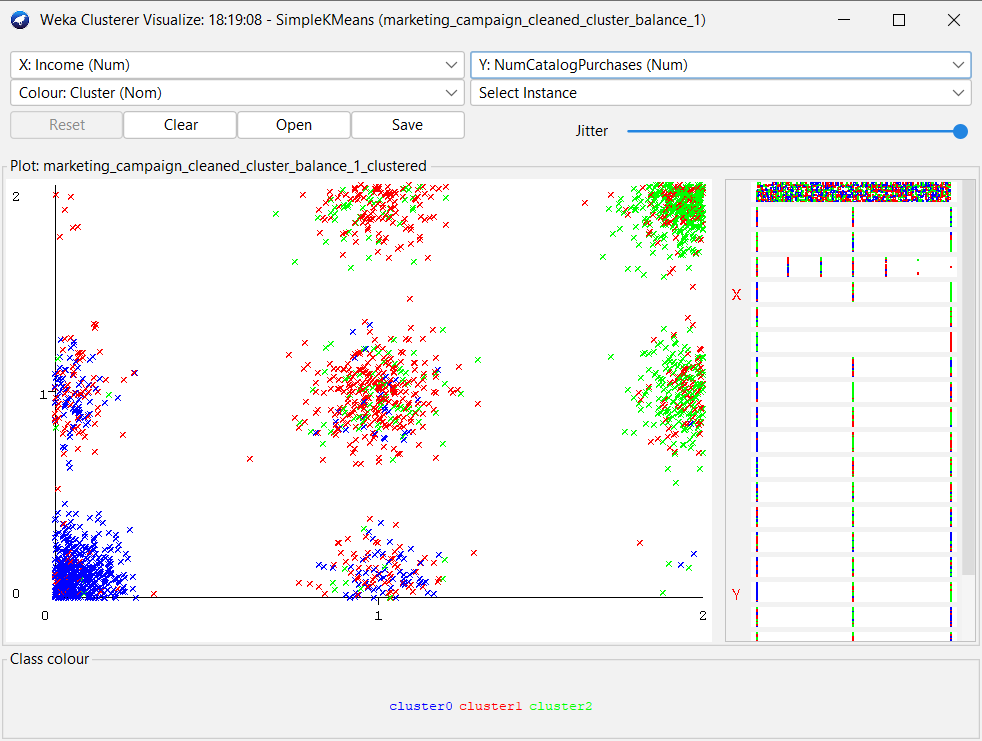
\includegraphics[scale=0.6]{imgs/cluster_income_catalog}
  \centering
  \caption{Income - NumCatalogPurchases}
  \label{NumCatalogPurchases}
\end{figure}

The figure\ref{NumCatalogPurchases} displays the distribution of income and the number of purchases made using catalogues. It appears that individuals with higher income tend to use catalogues to make purchases, while those with lower income tend to do the opposite.


\begin{figure}[H]
  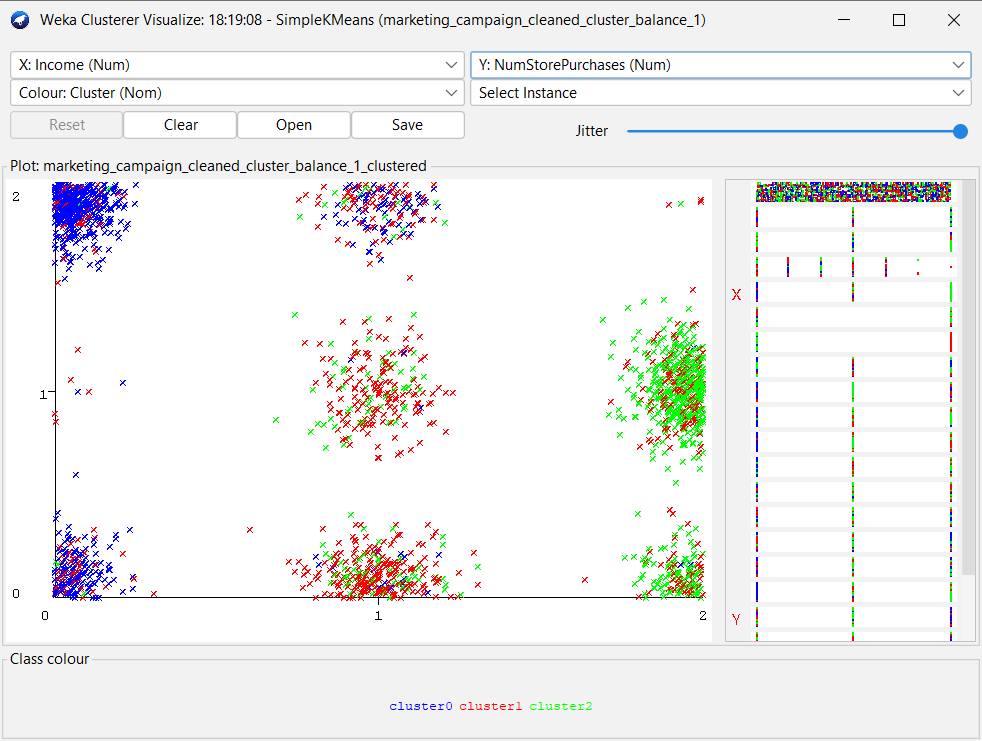
\includegraphics[scale=0.6]{imgs/cluster_income_store}
  \centering
  \caption{Income - NumStorePurchases}
  \label{NumStorePurchases}
\end{figure}

The figure\ref{NumStorePurchases} indicates that individuals with lower income tend to prefer purchasing items from stores, while those with higher income tend to make fewer purchases from stores.



\begin{figure}[H]
  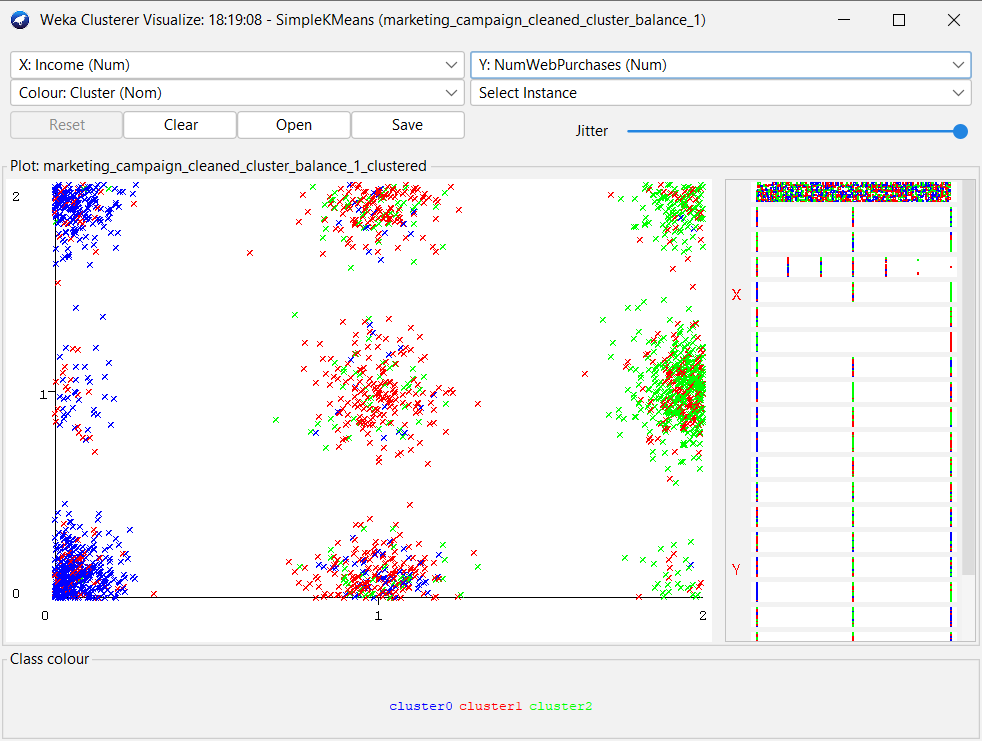
\includegraphics[scale=0.6]{imgs/cluster_income_webbuy}
  \centering
  \caption{Income - NumWebPurchases}
  \label{NumWebPurchases}
\end{figure}

The figure\ref{NumWebPurchases} shows that there are two extreme groups of lower Income: one that prefers to buy a great amount of items online and the other that does not. For the higher income class, most individuals prefer buying items online.

\begin{figure}[H]
  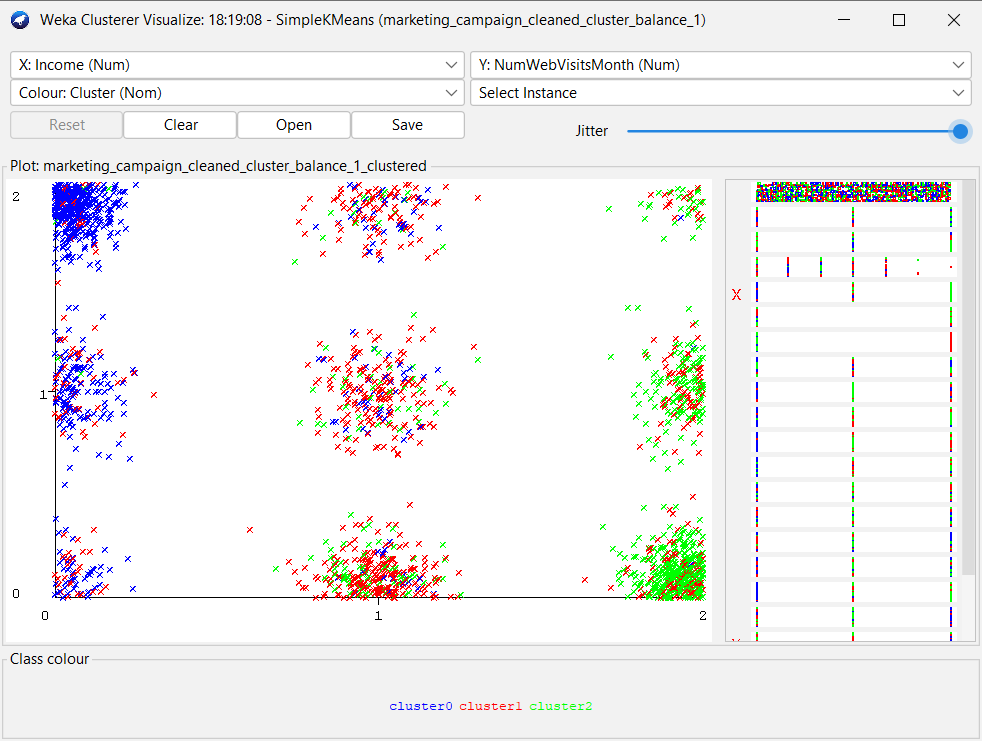
\includegraphics[scale=0.6]{imgs/cluster_income_webvisit}
  \centering
  \caption{Income - number of visits to company’s web site}
  \label{VisitPermonths}
\end{figure}

The figure\ref{NumWebPurchases}, it appears that individuals with lower income tend to visit a greater amount of stores, while those with higher income tend to do the opposite.